
\exercise{Simple Taylor expansion}{2}\label{exGeneratingSimple}Taylor expand the function 
\eqn{
f(x)=\frac{1}{x+1}
}
up to linear order around $x=0$.

\solution
We consider 
\eq{
f(x)=\frac{1}{1+x}.
}
We will need the derivative 
\eq{
f'(x) = \partial_x \frac{1}{x+1} = -\frac{1}{(x+1)^2} 
}

Using the equations from the chapter we can now compute the coefficients. The zeroth-order (constant) coefficient of the expansion is 
\eq{
c_0=f(0)=1.
}
The first-order (linear) is 
\eq{
c_1=f'(0) = -1
}
as well. Hence we can approximate 
\eq{
f(x)=\frac{1}{x+1} \approx 1-x = g(x).
}
Let's plot this along with the function to see that it works,
\begin{center}
    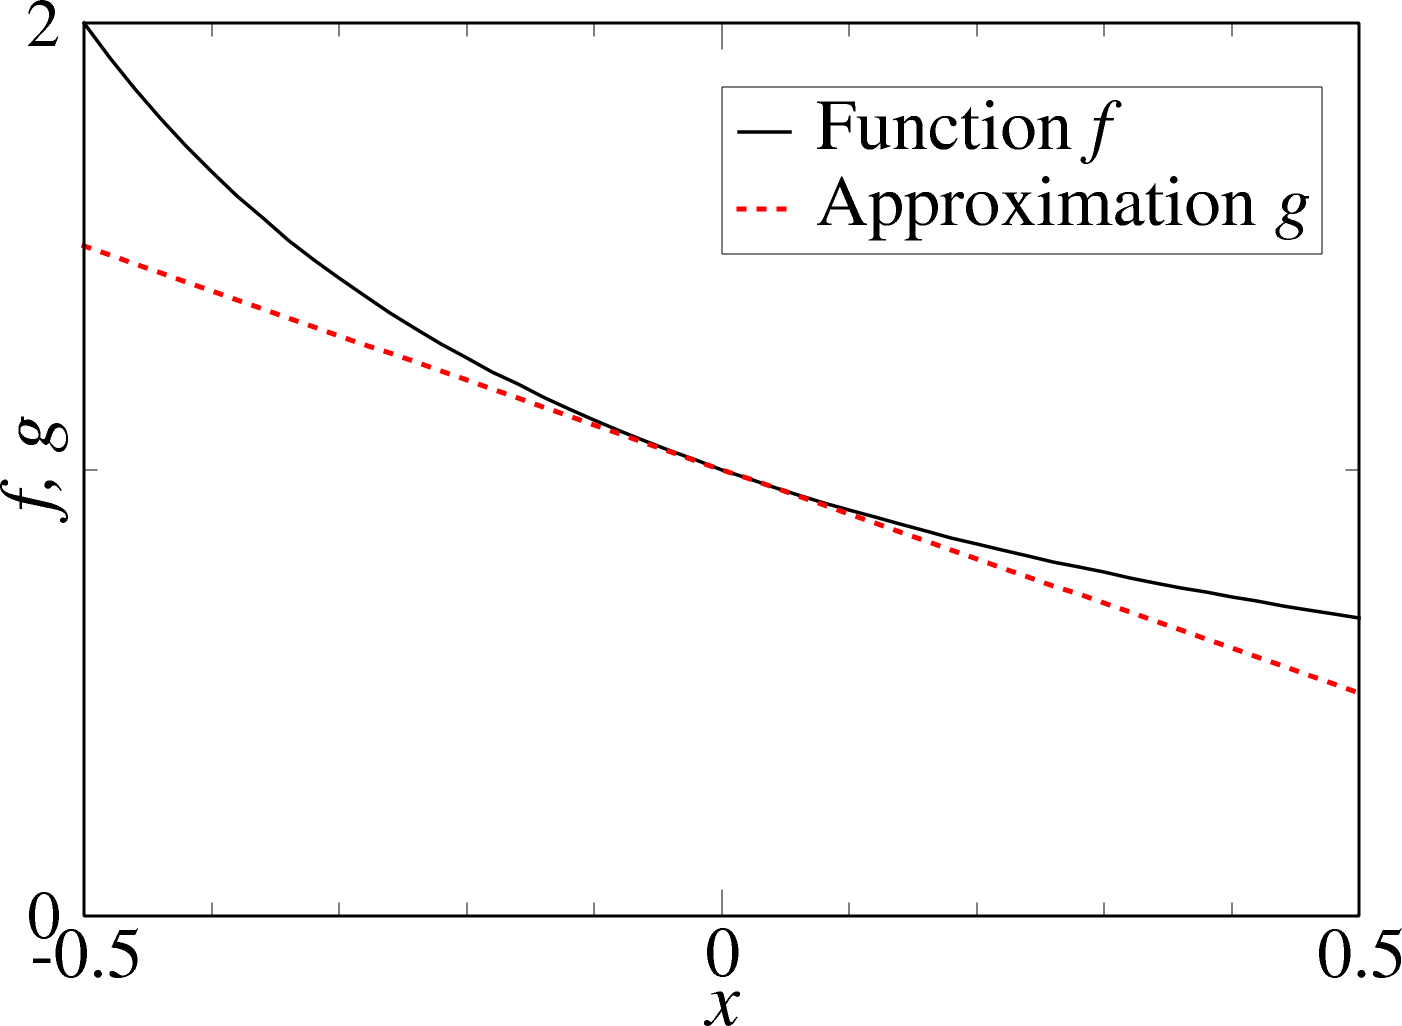
\includegraphics[width=0.6\textwidth]{approximation3}
\end{center}
